\documentclass[10pt]{article}
\usepackage[final]{graphicx}
\usepackage{amsfonts}

\topmargin -.5in
\textwidth 6.6in
\textheight 9in
\oddsidemargin 0in
\usepackage{color}
\newcommand{\arvind}[1]{{\color{red}{Arvind: {#1}}}}

\def\ds{\displaystyle}
\def\d{\partial}
\linespread{1.5}

\begin{document}

\subsection{Data processing}
\arvind{Describe what other preprocessing was done to the data.} 

%\subsubsection{Clean the AVHRR AOD data}

No matter what PM2.5 sites we use, we need to find the closest AOD coordinates to the PM2.5 sites, and then to match the sites data for each day. This requires us to search all the observations in AOD dataset. The AOD data are very large and we cannot put all the data in hundreds of files into one matrix. Besides, AOD data have lots of missing data. So we need to clean the AOD data first. 

Since the data we want to use are the data located on the west coast and Hawaii, first we used the longitude and latitude of the west coast and Hawaii to eliminate data from other locations that we won\rq t use. Then, we dropped all the missing data and also changed the original format of the data into more readable one. Finally, our AOD data looks like Table \ref{table3.1}. 

\subsection{PM$_{2.5}$ sites adjacent to AVHRR grids}
Since the coverage of the AOT data is over the oceans, and the PM$_{2.5}$ data is collected over the land, there is no direct overlap between the two datasets. In order to compare the two data sets, we adopt the following strategy. First, of all the PM$_{2.5}$ measurement sites, we identify those that are close to the coast. Figure~\ref{graph3} shows the geographical location of all the PM$_{2.5}$ sites, whereas Figure~\ref{graph4} shows the geographical locations to $13$ locations -- four of these are found in California, whereas the rest can be found in Hawaii.  In the rest of this report, we focus on only these $13$ locations. \arvind{Can you also mention that we only chose overlapping temporal data.}


%As AVHRR satellites can only get the aerosol optical depth (AOD) from oceans and PM$_{2.5}$ data are from lands, our strategy for identifying PM$_{2.5}$ sites is to choose the ones that are as close to the coast as possible.  The sites were chosen due to their proximity to the west coast. 

\begin{figure}[ht!]
\centering
\includegraphics[width = 90mm]{ALLPMsites.png}
\caption{\arvind{Please fill in the caption}}
\label{graph3}
\end{figure}




\begin{figure}[ht!]
\centering
\includegraphics[width = 90mm]{PMsites.png}
\caption{\arvind{The figure only shows the California locations, can the figure include the Hawaii sites as well? This map could also be zoomed in further. Also add a caption.}}
\label{graph4}
\end{figure}




\subsection{Analzing PM$_{2.5}$ trends}
One method we used to analyze trends in the PM$_{2.5}$ data was to make an animation to show the change in the concentration of PM$_{2.5}$  over time. The animation plots points at each site where the PM$_{2.5}$ data was collected, with color varying depending on the intensity of the reading, with darker colors indicating a larger concentration of PM$_{2.5}$. 

%%%%%%%%%%%%%%%%%%%%%%%%%%%%%%%%%%%%%%%%%%%
%%%%%%%Tuo1
To figure out whether we can use previous PM2.5 value to predict future PM2.5 value, we decide to conduct time series analysis. We focus our attention on the PM2.5 site which located at latitude 33.79236 and longitude -118.175 ( It is really close to Long Beach). We collect monthly average PM2.5 concentration value from Jan 2004 to Dec 2014 and plot the time series in the figure below.

\begin{figure}[ht!]
\centering
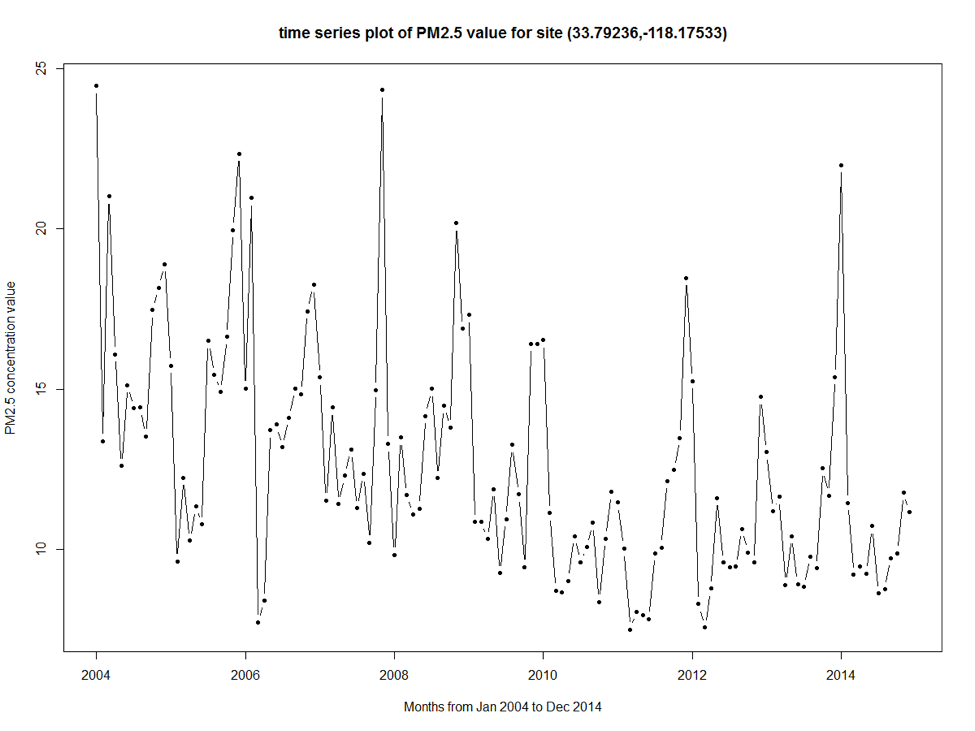
\includegraphics[width = 90mm]{ts1.png}
%\caption{}
%\label{graph4}
\end{figure}

There is a slightly downward trend over time about this time series and there seems to exist seasonality. We decide to use two different methods to fit the time series model. One is Holt-Winters Exponential Smoothing. Exponential smoothing is a very popular scheme to produce a smoothed time series and it assigns exponentially decreasing weights as the observations get older. Holt-Winters Exponential Smoothing can be used to make short-term forecasts on a time series that can be described using an additive model with increasing or decreasing trend and seasonality. The second one is ARIMA model. ARIMA is the short for autoregressive integrated moving average. This model can be fitted to time series data either to better understand the data or to predict future points in the series. For the ARIMA method, we firstly adjust the time series by subtracting the estimated seasonal component and then apply the model to the adjusted series.

%%%%%%end_Tuo1
%%%%%%%%%%%%%%%%%%%%%%%%



\arvind{The results of the experiments should be discussed in the next section}.
After analyzing this data we noticed (insert conclusion here... talk about it more...). The animation is available online (insert website-github?).

\subsection{Relationships between AVHRR AOD and surface PM$_{2.5}$}
We noticed that there was a huge difference between the  $13$ sites we identified along the West Coast and the sites located on Hawaii. The sites on Hawaii are unique because Hawaii is surrounded on water. Thus we decided to build models separately for both the sites along the West Coast and the sites on Hawaii. 

\subsubsection{Only AOD data}
Since there are many meteorological parameters varying from day to day, our statistical model must have the variability of the date. For each location, there are many different geographical properties, so our model must have the variability of sites. Therefore we used mixed effects model to fit this relationship:

$$PM_{ij} = \alpha + \beta\times AOD_{ij} + s_i + d_j+ \epsilon_{ij}, $$

where $PM_{ij}$ is the $PM_{2.5}$ concentration at a spatial site $i$ on a specific day $j$, $\alpha$ is the fixed intercept, $\beta$ is the fixed slope, $AOD_{ij}$ is the AOD value at a spatial site $i$ on a specific day $j$, $s_i\sim N(0, \sigma_s^2)$ is the random intercept of site $i$, $d_j\sim N(0, \sigma_d^2)$ is the random intercept of a specific day $j$, and $\epsilon_{ij}\sim N(0, \sigma^2)$ is the error term at site $i$ on a day $j$.

\subsubsection{AOD data and wind data}


\begin{table}[!h]
\centering
\begin{tabular}{|c|c|c|c|}
\hline 
Date & lat\_aot & long\_aot & aot\\
\hline
2000-01-25 & 30 & -126.6 & -0.0836133733391762 \\
\hline
$\cdots$ & $\cdots$ & $\cdots$ & $\cdots$\\
\hline
\end{tabular}
\caption{AOD data}
\label{table3.1}
\end{table}

\subsubsection{Match the AOD data with the PM2.5 data}
As we are trying to find the relationships between AOD and PM2.5, we need to keep all the date the same, and locations closest. After matching these two datasets, we got the following as in Table {table3.2}.

\begin{table}[!h]
\centering
\begin{tabular}{|c|c|c|c|c|c|c|}
\hline 
Date & lat\_pm & long\_pm & pm & lat\_aot & long\_aot & aot\\
\hline
2006-12-28 & 40.776944 & -124.1775 & 17.8 & 40.9 & -124.3 & 0.043815478682518\\
\hline
$\cdots$ & $\cdots$ & $\cdots$ & $\cdots$ & $\cdots$ & $\cdots$ & $\cdots$\\
\hline
\end{tabular}
\caption{AOD and PM2.5 match data}
\label{table3.2}
\end{table}


\end{document}